\documentclass[a4paper,11pt]{article}
\usepackage[T1]{fontenc}
\usepackage[utf8]{inputenc}
\usepackage[francais]{babel}
\usepackage{lmodern}
\usepackage{amsmath}
\usepackage{graphicx}
\usepackage{multicol}
\usepackage{color}
\usepackage{array}
\setlength\abovecaptionskip{0.10ex}
\RequirePackage{graphicx}
\DeclareGraphicsExtensions{.pdf,.jpg,.png,.JPG}
\RequirePackage{float}
\usepackage{titling}
\setlength{\droptitle}{-4cm}
\usepackage{fullpage}
\usepackage{amsfonts}




\title{Rapport SY09 TP04 - Théorie de la décision}
\author{Jean-Baptiste Audibert \& Yueqing Qin}
\date{\today} 

\begin{document}
\maketitle

\section{Etude de la règle de Bayes} 

\noindent Dans cet exercice, nous allons étudier la règle de Bayes pour un échantillon de la population, répartis en deux classe $\omega_1$ et $\omega_2$, de proportions $\pi_1$ et $\pi_2 = 1 - \pi_1$. Ces classes sont issus de distributions gaussiennes bivariées :  \\

\begin{itemize}
\item Classe $\omega_1 \  \sim \ \mathcal{N}( \mu_1, \Sigma_1)$,
\item Classe $\omega_2 \  \sim  \ \mathcal{N}( \mu_2, \Sigma_2)$. \\
\end{itemize}

\noindent Où $\pi_1$, $\pi_2$, $\mu_1$, $\mu_2$, $\Sigma_1$ et $\Sigma_2$ varient.
\noindent On étudie 5 cas, pour chacun on génère un nuage échantillon de taille totale $n = 1000$, on calcule la frontière entre les deux classes, et on affiche le nuage de points ainsi que la frontière associée.

\subsection{Equation des frontières}

\noindent Pour retrouver l'équation des frontières, on calcule pour chaque cas et pour chaque classe la \textbf{fonction discriminante} $g_k(x)$. L'expression de celle ci, pour différentes classes, issus de distributions gaussiennes bivariées, de paramètres $\mu_k$ et $\Sigma_k$ différents est la suivante : 

\begin{center}
$g_k(x) = -\frac{1}{2}(x-\mu_k)' \Sigma_k^{-1}(x-\mu_k) - \frac{1}{2}$ln$($det$\Sigma_k) + $ln$\pi_k - \frac{p}{2}$ln$(2\pi).$ (1)
\end{center}

\subsubsection{Cas 1}
\noindent On se place dans le cas où les variances $\Sigma_1$ et $\Sigma_2$ sont égales - \textbf{hypothèse d'homoscédasticité} : 

$g_1(x) = -\frac{1}{2}(x_1  \ x_2) \begin{pmatrix}1&0\\0&1\end{pmatrix}\left (\begin{array}{ccc}x_1 \\x_2\end{array}\right ) + $ln$\pi_1$ \\ \\
$g_2(x) = -\frac{1}{2}(x_1-1  \ \ x_2-1)  \begin{pmatrix}1&0\\0&1\end{pmatrix}\left (\begin{array}{ccc}x_1-1 \\x_2-1\end{array}\right ) + $ln$\pi_2$\\

\noindent Pour obtenir l'équation de la frontière, on pose 
 \begin{center}
   $$ 
   \begin{array}{rcl}
  g_1(x) &=& g_2(x) \\ \\
  -\frac{1}{2}x_1^2 -\frac{1}{2} x_2^2 + $ln$\pi_1  &=&  -\frac{1}{2} (x_1 -1)^2 - \frac{1}{2} (x_2 - 1)^2 + $ln$ \pi_2 \\ \\
  x_1^2 + x_2^2 &=& (x_1^2 - 2x_1 + 1) + (x_2^2 - 2x_2 + 1) +$ln$\left(\frac{\pi_2}{\pi_1}\right) \\ \\
  x_1 &=& 1 - x_2 + $ln$ \left(  \frac{\pi_2}{\pi_1}\right) = 1- x_2\\
	       \end{array}
   $$
\end{center}

\noindent C'est l'équation d'une \textbf{droite}.

\subsubsection{Cas 2}

\noindent On réalise le même développement, mais cette fois ci $\pi_1 \ne \pi_2$ : 
\begin{center}
   $$ 
   \begin{array}{rcl}
  x_1 &=& 1 - x_2 + $ln$ \left(\frac{\pi_2}{\pi_1}\right)\\ \\
  x_1 &=& 1 - x_2 + $ln$\left( \frac{0,1}{0,9} \right) \\ \\
  x_1 &\approx& -x_2 - 1,2 \\
	       \end{array}
   $$
\end{center}

\noindent Qui est également l'équation d'une \textbf{droite}.

\subsubsection{Cas 3}

\noindent On obtient la même équation que dans le \textit{Cas 1}, l'équation d'une \textbf{droite}. :

\begin{center}
$x_1 = 1  - x_2$ \\
\end{center}

\subsubsection{Cas 4}
\noindent On repart cette fois ci de l'équation (1) pour trouver les fonctions discriminantes :

\begin{center}
$g_1(x) = -\frac{1}{2} (x_1 - 1)^2 - \frac{1}{2}(x_2 - 1)^2 + $ln$\pi_1 - $ln${2\pi}$ \\  
$g_2(x) = -\frac{1}{10}  (x_1 - 1)^2 - \frac{1}{10} (x_2 - 1)^2 -\frac{1}{2}$ln$(25)+ $ln$\pi_2 - $ln${2\pi}$ \\
\end{center}

\noindent Soit l'équation de la frontière :

\begin{center}
$(x_1 - 1)^2 + (x_2 - 2)^2 = \frac{5}{4}$ln$(25) + \frac{5}{2}$ln$\left(\frac{\pi_2}{\pi_1}\right)$
\end{center}

\noindent Qui est donc un \textbf{cercle}, de centre $\mu = (1,1)^T$ et de rayon  $r=\frac{5}{4}$ln$(25) + \frac{5}{2}$ln$\left(\frac{\pi_2}{\pi_1}\right)$

\subsubsection{Cas 5}
\noindent On utilise la même démarche que dans le Cas 4 et on obtient 

\begin{center}
   $$ 
   \begin{array}{rcl}
  -\frac{1}{2} + $ln$(\pi_1) &=& -\frac{4}{6} (x_1^2 - x_1 x_2^2) - \frac{2}{3} (x_1 + x_2) -\frac{2}{3} -\frac{1}{2}$ln$\left(\frac{3}{4} \right) + $ln$(\pi_2) \\ \\
  
	       \end{array}
   $$
\end{center}

\noindent Ceci est l'équation d'une \textbf{ellipse}.

\noindent Une fois les frontières calculées, on affiche les échantillons et les frontières :

\InsertFig{ex1}

\subsection{Etude de la probabilité d'erreur}

\noindent Les probabilités d'erreur théoriques nous sont données par la probabilité d'erreur de Bayes et la borne de Bhattacharyya (l'un ou l'autre selon les hypothèses), avec les paramètres $c$, le nombre de classes, $\Sigma_k$, les matrice de variance, $\phi$ la fonction de répartition de la loi normale,  $\Delta = (\mu_2 - \mu_1)' \Sigma^{-1}(\mu_2 - \mu_1)$ le carré de la distance de Mahalanobis, et \newline $\Delta_B^2 = \frac{1}{8}(\mu_2 - \mu_1)' \left( \frac{\Sigma_1 + \Sigma_2}{2} \right)^{-1} (\mu_2 - \mu_1) + \frac{1}{2}$ln$\frac{det\frac{\Sigma_1 + \Sigma_2}{2}}{\sqrt{det\Sigma_1 det \Sigma_2}}$, le carré de la distance de Bhattacharyya entre les deux classes \\

\begin{itemize}
\item Probabilité d'erreur de Bayes:  $c=2$, $\Sigma_k = \Sigma$ : \\ 
$\displaystyle \epsilon^{*} = \phi \left( \frac{ ln( \pi_1 /  \pi_2) - \Delta^2/2 } {\Delta}\right) \pi_2 + \left[ 1 - \phi \left( \frac{ln(\pi_1/\pi_2) + \Delta^2/2}{\Delta} \right) \right] \pi_1$ \\ \\ 
\item Borne de  Bhattacharyya (borne supérieur de l'erreur de Bayes) $c=2$ et $\Sigma_k$ quelconques  : \\ 
$\epsilon^* = \sqrt{\pi_1 \pi_2} e^{-\Delta_B^2} $ \\
\end{itemize}

\noindent On obtient alors les résultats suivants :

\begin{center}
\begin{tabular}{|l|c|c|}
\hline
Cas & Réalisation & Erreur théorique  \\
\hline
Cas 1 & $0,222$ & $0,228$  \\
Cas 2 & $0,312$ & $0,223$ \\
Cas 3 & $0,204$ & $0,183$ \\
Cas 4 & $0,390$ & $0,393$ \\
Cas 5 & $0,335$ & $0,357$ \\ 
\hline
\end{tabular}
\end{center}
\\ \\

\section{Analyse discriminante sur les données Crabes}

\subsection{Présentation des fonctions} 

\noindent La fonction \textbf{lda} permet de réaliser \textit{directement} \textbf{l'analyse discriminante linéaire}. \\

\noindent La fonction \textbf{qda} permet de réaliser \textit{directement} textbf{l'analyse discriminante quadratique}. \\

\noindent La fonction \textbf{contour} permet de tracer, sur un graphique, les lignes de niveaux associées à une fonctions dépendant de deux variables. \\

\noindent Enfin, la fonction \textbf{sample} permet de tirer, de manière aléatoire un sous échantillon issu d'un échantillon existant. \\ 

\noindent La différence entre les fonctions \textbf{predict} et \textbf{predict.lda} réside dans le fait que la première est utilisée selon le type de données étudié, alors que  \textbf{predict.lda} réalise le même travaille mais uniquement pour des données issues de la fonction \textbf{lda}. 

\subsection{Analyse discriminante linéaire et quadratique}

\noindent On réalise tout d'abord l'analyse discriminante linéaire sur l'ensemble des crabes, et on affiche les points à partir des variables réduites \textit{FL1} et \textit{RW1}, qui permettent de déterminer le sexe. On a les résultats suivants : 


\begin{figure}[H]
\begin{center}
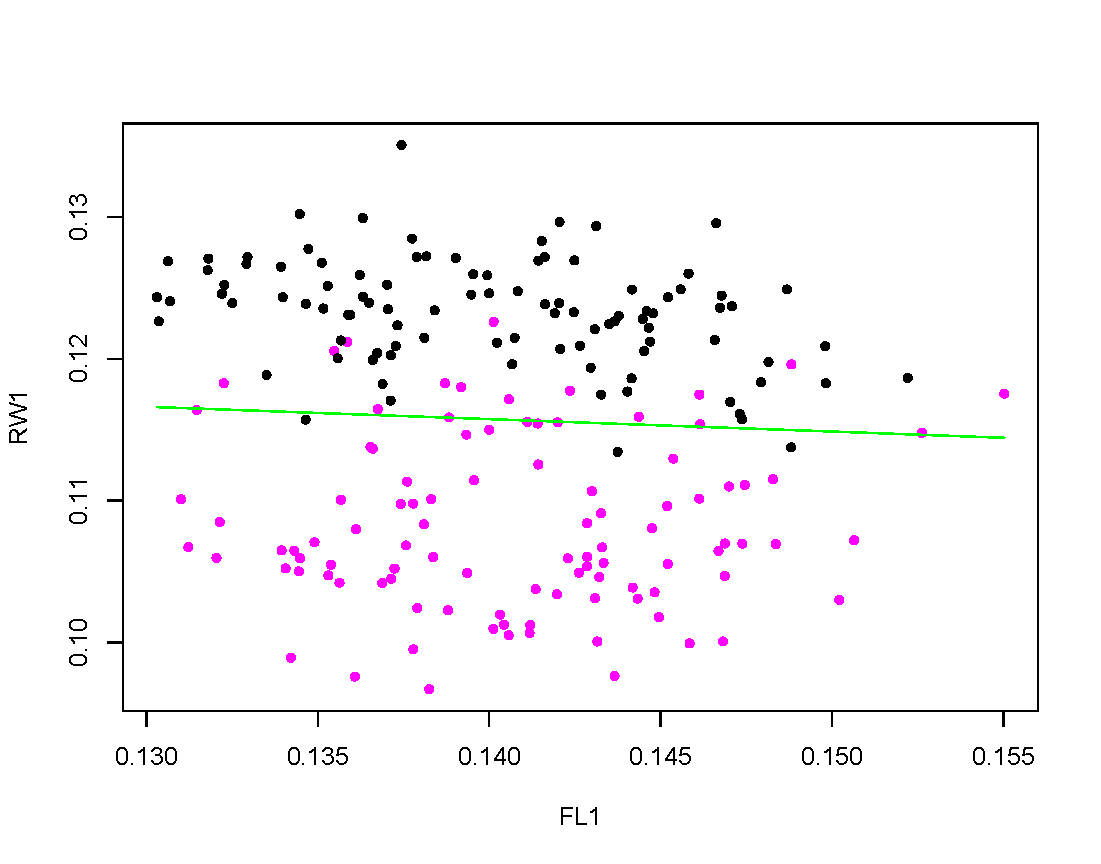
\includegraphics[width=.6\textwidth]{img/lda}
\caption{Réalisation de l'analyse discriminante linéaire sur les données crabes}
\end{center}
\end{figure}

\noindent Ainsi qu'une erreur de $9.5 \%$. 

\noindent Pour l'analyse discriminante quadratique, on a les résultats suivants : 

\begin{figure}[H]
\begin{center}
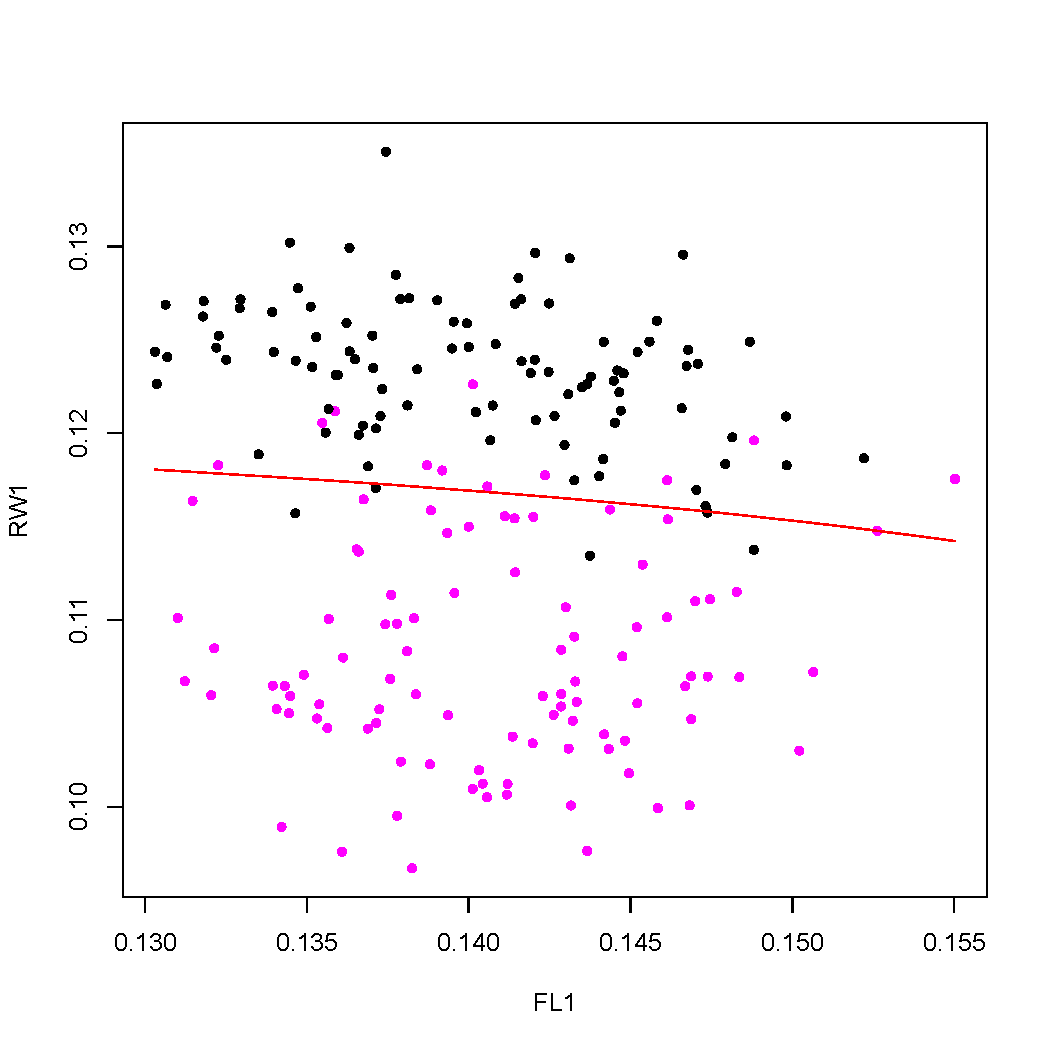
\includegraphics[width=.6\textwidth]{img/qda}
\caption{Réalisation de l'analyse discriminante quadratique sur les données crabes}
\end{center}
\end{figure}

\noindent Et une erreur de $8.5 \%$. On remarque que ces erreurs sont très proches, car les frontières de décisions sont également proches. Ceci s'explique par le fait que les deux classes sont \textbf{linéairement séparables}, impliquant que l'analyse quadratique, analyse sans hypothèse qui pourrait fausser l'analyse discriminante, n'apporte pas des résultat plus pertinents.

\subsection{Estimation de l'erreur d'apprentissage avec un ensemble de test}

\noindent On souhaite désormais réalise l'analyse discriminante avec un \textbf{échantillon d'apprentissage} et un \textbf{échantillon de test} distincts. On sélectionne tout d'abord $\frac{2}{3}$ des données \textit{crabs} pour l'échantillon d'apprentissage, et les $\frac{1}{3}$ restants pour l'échantillon de test. On répète ce processus pour différentes proportions de découpages et on obtient les résultats : 

\begin{center}
\begin{tabular}{|l|c|c|c|}
\hline
Proportion & Nombre d'estimation & LDA & QDA  \\ 
\hline
$\frac{2}{3}$-$\frac{1}{3}$& $1$ & $3,91\%$ & $4\%$ \\
$\frac{2}{3}$-$\frac{1}{3}$& $200$ & $2,98\%$  & $2.35\%$\\
$\frac{1}{2}$-$\frac{1}{2}$& $1$ & $5,5\%$ & $3,25\%$ \\ 
$\frac{1}{2}$-$\frac{1}{2}$& $200$ & $4,58\%$ & $3,92\%$ \\ 
\hline
\end{tabular}
\end{center}
\\ \\

\noindent On voit ici tout d'abord que la répétition du processus d'analyse permet d'approcher au mieux l'erreur d'apprentissage. De plus, on observe toujours que les résultats des analyses discriminante linéaire et quadratique sont proches, et que cette dernière n'apporte pas de résultats plus précis. Enfin, on observe que plus l'échantillon d'apprentissage est grand, moins l'erreur est importante.

\section{Etude des différents classifieurs}

\subsection{Estimation des paramètres du modèle}

\subsubsection{Cas 1}

On suppose $\pi_1 = \pi_2$ et $\Sigma_1 = \Sigma_2 = \sigma^2 I$, et on estime les paramètres :  \\

\begin{itemize}
\item $\hat\pi_1 = \frac{n_1}{n} = 0.5$, $\hat\pi_2 = 0.5$ \\
\item $\hat\mu_1 = \frac{1}{n_1} \displaystyle \sum^{n}_{i=1} t_{i1} x_i = (0.64,0.50)^T$, $\hat\mu_2 = (2.12,2)^T$\\
\item $S = \frac{1}{n-c} \displaystyle \sum^{c}_{k=1} (n_k - 1) S_k$\\
$S = \begin{pmatrix}1.38&-0,66\\-0,66&0.86\end{pmatrix} $, d'où l'estimateur $\hat\sigma^2 = \frac{1}{2}trace(S) = 1,12$

\end{itemize}

\subsubsection{Cas 2}

\noindent On suppose $\Sigma_1 = \Sigma_2$, et on estime les paramètres :  \\

\begin{itemize}
\item $\hat\pi_1 = \hat\pi_2 = 0.5$ \\ 
\item $\hat\mu_1 = (0.64,0.50)^T$, $\hat\mu_2 = (2.12,2)^T$\\
\item On utilise l'estimateur sans biais pour estimer la variance : \\
	$S = \frac{1}{n-c} \displaystyle \sum^{c}_{k=1} (n_k - 1) S_k$ avec $S_k = \frac{n_k}{n_k-1} \hat\Sigma_K$ \\
	$S = \begin{pmatrix}1.38&-0.66\\-0.66&0.86\end{pmatrix}$
	

\end{itemize}

\subsubsection{Cas 3}

\begin{itemize}
\item $\hat\pi_1 = \frac{n_1}{n} = 0.5$, $\hat\pi_2 = 0.5$ \\
\item $\hat\mu_1 = (0.64,0.50)^T$, $\hat\mu_2 = (2.12,2)^T$\\
\item $S_1 = \frac{n_1}{n_1 -1}diag(\hat\Sigma_1) = \begin{pmatrix}1.45&0\\0&1.18\end{pmatrix}$\\
$S_2=\begin{pmatrix}1.31&0\\0&0.535\end{pmatrix}$

\end{itemize}

\subsubsection{Cas 4}

\begin{itemize}
\item $\hat\pi_1 = \frac{n_1}{n} = 0.5$, $\hat\pi_2 = 0.5$ \\
\item $\hat\mu_1 = (0.64,0.50)^T$, $\hat\mu_2 = (2.12,2)^T$\\
\item On utilise l'estimateur sans biais pour estimer la variance : \\$S_1 = \frac{n_1}{n_1 -1}\hat\Sigma_1 = \begin{pmatrix}1.45&-0.91\\-0.91&1.18\end{pmatrix}$\\
$S_2=\begin{pmatrix}1.31&-0.42\\-0.42&0.535\end{pmatrix}$
\end{itemize}



\subsection{Lien avec les différents classifeurs}

\begin{itemize}
\item Le cas 1 correspond au \textbf{classifieur euclidien}, \\
\item Le second cas correspond à \textbf{l'analyse discriminante linéaire}\\
\item Le troisième cas correspond au \textbf{classifieur bayésiens naïfs}\\
\item Le dernier à \textbf{l'analyse discriminante quadratique}\\
\end{itemize}

\subsection{Fonction discriminantes}

\noindent L'expression de la fonction de décision nous est donné par : 

\begin{center}
$g(x) = \frac{1}{2}(x-\mu_1)' \Sigma_1^{-1}(x-\mu_1) - \frac{1}{2}(x-\mu_2)'\Sigma_2^{-1}(x-\mu_2) + \frac{1}{2}$ln$\frac{|\Sigma_1|}{|\Sigma_2|} - \frac{\pi_1}{\pi_2}$
\end{center}

\noindent On l'applique dans les différents cas, et on trouve les résultats suivants : 

\subsection{Classifieur euclidien}

\noindent $g(x) = 1,48 x_1 + 1,5 x_2 - 3,92$

\subsection{Analyse disciminante linéaire}

\noindent $g(x) = 3.87x_1 + 5,23x_2 - 11,87$

\subsection{Classifieur bayésiens naïfs}

\noindent $g(x) = -0,04x_1^2 -0,52x_2^2 + 1,18x_1 + 3,35 - 4,79$

\subsection{Analyse discriminante quadratique}

\noindent $g(x) = 0,17 x_1^2 - 0,41 x_2^2 + 0,26x_1x_2 + 2,31 + 5,12x_2 - 9,48$ 


\end{document}